\documentclass{article}
\usepackage{tikz}
\usepackage{adjustbox}
\usetikzlibrary{shapes.geometric, arrows, positioning, arrows.meta, fit, decorations.pathreplacing, decorations.pathmorphing, calc}

% Define arrow color
\colorlet{highlightArrowColor}{red}

\begin{document}

\begin{figure}[ht]
  \begin{center}
  \caption{Illustrative Example of a Hierarchical Task-Based Production}
  \label{fig:hierarchical_production}
  \vspace{0.5cm}
  
  \begin{adjustbox}{center,trim=0pt 0pt 0pt 0pt,clip,margin=-2cm 0cm}
  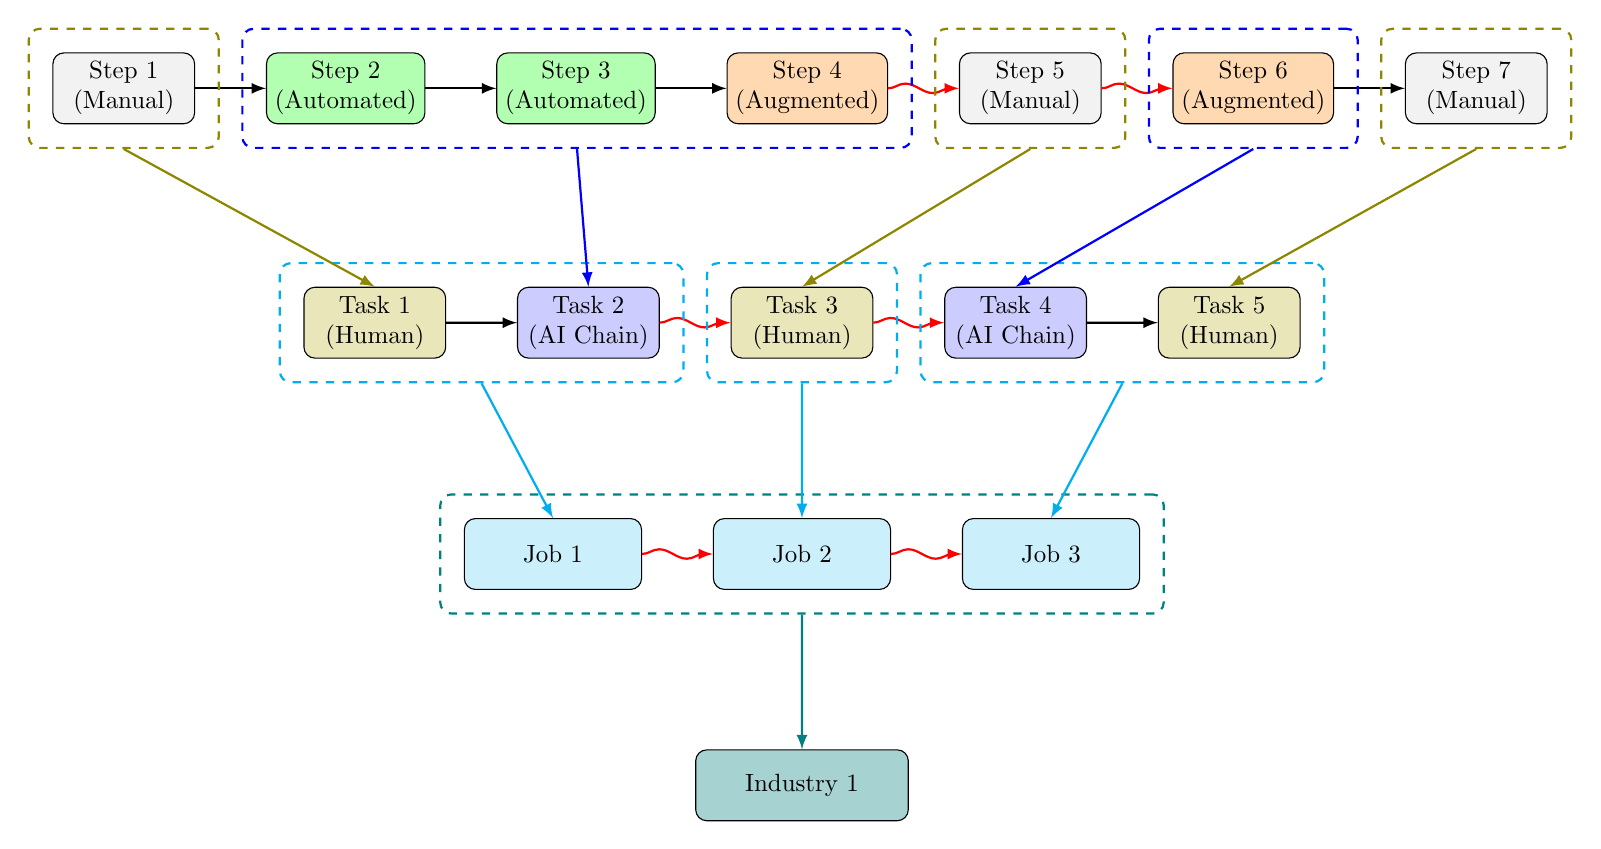
\begin{tikzpicture}[scale=0.9, transform shape,
    node distance=0.35cm and 1cm,
    every node/.style={rectangle, rounded corners, draw, align=center, minimum width=2cm, minimum height=1cm},
    manual/.style={fill=gray!10},
    automated/.style={fill=green!30},
    augmented/.style={fill=orange!30},
    dashedbox/.style={draw, rectangle, rounded corners, dashed, inner sep=0.3cm, line width=0.8pt},
    humanbox/.style={rectangle, rounded corners, draw, align=center, minimum width=2cm, minimum height=1cm, fill=olive!20}, % changed to olive
    aibox/.style={rectangle, rounded corners, draw, align=center, minimum width=2cm, minimum height=1cm, fill=blue!20},
    jobbox/.style={rectangle, rounded corners, draw, align=center, minimum width=2.5cm, minimum height=1cm, fill=cyan!20},
    industrybox/.style={rectangle, rounded corners, draw, align=center, minimum width=3cm, minimum height=1cm, fill=teal!35},
    >=latex
  ]

    % Top layer (Steps)
    \node[manual] (S1) {Step 1\\(Manual)};
    \node[automated, right=of S1] (S2) {Step 2\\(Automated)};
    \node[automated, right=of S2] (S3) {Step 3\\(Automated)};
    \node[augmented, right=of S3] (S4) {Step 4\\(Augmented)};
    \node[manual, right=of S4] (S5) {Step 5\\(Manual)};
    \node[augmented, right=of S5] (S6) {Step 6\\(Augmented)};
    \node[manual, right=of S6] (S7) {Step 7\\(Manual)};

    % Arrows between steps (specific arrows as curly lines)
    \draw[->, thick] (S1) -- (S2);
    \draw[->, thick] (S2) -- (S3);
    \draw[->, thick] (S3) -- (S4);
    \draw[->, thick, highlightArrowColor, decorate, decoration={snake, amplitude=.6mm, segment length=7mm}] (S4) -- (S5);
    \draw[->, thick, highlightArrowColor, decorate, decoration={snake, amplitude=.6mm, segment length=7mm}] (S5) -- (S6);
    \draw[->, thick] (S6) -- (S7);

    % Dashed boxes (top layer, colors updated)
    \node[dashedbox, draw=olive, fit=(S1)] (DS1) {};
    \node[dashedbox, draw=blue, fit=(S2)(S3)(S4)] (DS2-4) {};
    \node[dashedbox, draw=olive, fit=(S5)] (DS5) {};
    \node[dashedbox, draw=blue, fit=(S6)] (DS6) {};
    \node[dashedbox, draw=olive, fit=(S7)] (DS7) {};

    \path (S1.west) -- (S7.east) coordinate[midway] (CenterTop);

    % Middle layer (Tasks, human task color updated)
    \node[humanbox, below=2.8cm of CenterTop, xshift=-6cm] (T1) {Task 1\\(Human)};
    \node[aibox, right=of T1] (T2) {Task 2\\(AI Chain)};
    \node[humanbox, right=of T2] (T3) {Task 3\\(Human)};
    \node[aibox, right=of T3] (T4) {Task 4\\(AI Chain)};
    \node[humanbox, right=of T4] (T5) {Task 5\\(Human)};

    % Arrows between tasks (specific arrows as curly lines)
    \draw[->, thick] (T1) -- (T2);
    \draw[->, thick, highlightArrowColor, decorate, decoration={snake, amplitude=.6mm, segment length=7mm}] (T2) -- (T3);
    \draw[->, thick, highlightArrowColor, decorate, decoration={snake, amplitude=.6mm, segment length=7mm}] (T3) -- (T4);
    \draw[->, thick] (T4) -- (T5);

    % Dashed boxes (middle layer)
    \node[dashedbox, draw=cyan, fit=(T1)(T2)] (DT1-2) {};
    \node[dashedbox, draw=cyan, fit=(T3)] (DT3) {};
    \node[dashedbox, draw=cyan, fit=(T4)(T5)] (DT4-5) {};

    % Job layer nodes
    \node[jobbox, below=2.25cm of T3] (J2) {Job 2};
    \node[jobbox, left=of J2] (J1) {Job 1};
    \node[jobbox, right=of J2] (J3) {Job 3};

    % Arrows between jobs (specific arrows as curly lines)
    \draw[->, thick, highlightArrowColor, decorate, decoration={snake, amplitude=.6mm, segment length=7mm}] (J1) -- (J2);
    \draw[->, thick, highlightArrowColor, decorate, decoration={snake, amplitude=.6mm, segment length=7mm}] (J2) -- (J3);

    % Dashed box job layer
    \node[dashedbox, draw=teal, fit=(J1)(J2)(J3)] (JobsBox) {};

    % Industry layer
    \node[industrybox, below=2.25cm of J2] (Industry) {Industry 1};

    % Arrows connecting layers (unchanged)
    \draw[->, thick, teal] (JobsBox.south) -- (Industry.north);
    \draw[->, thick, cyan] (DT1-2.south) -- (J1.north);
    \draw[->, thick, cyan] (DT3.south) -- (J2.north);
    \draw[->, thick, cyan] (DT4-5.south) -- (J3.north);

    \draw[->, thick, olive] (DS1.south) -- (T1.north);
    \draw[->, thick, blue] (DS2-4.south) -- (T2.north);
    \draw[->, thick, olive] (DS5.south) -- (T3.north);
    \draw[->, thick, blue] (DS6.south) -- (T4.north);
    \draw[->, thick, olive] (DS7.south) -- (T5.north);

  \end{tikzpicture}
  \end{adjustbox}
  \end{center}

\footnotesize{\emph{Notes:} This figure provides an illustrative example of a hierarchical production process consisting of four layers in a representative industry. The top layer includes \(m=7\) Steps categorized into Manual (gray), Automated (green), and Augmented (orange) modes of execution. Steps are grouped by dashed boxes colored according to their corresponding Task boxes in the layer below. The second layer aggregates Steps into \(n=5\) Tasks, labeled as Human-executed tasks (olive) or AI Chain tasks (blue) depending on the mode of execution. Dashed boxes in this layer are colored cyan to correspond with the Jobs layer below. The third layer consolidates Tasks into \(l=3\) Jobs, represented in cyan-colored boxes. Finally, the bottom layer represents the Industry level (teal), encapsulating the entire production structure. Vertical arrows show the aggregation from individual Steps through Tasks and Jobs, down to the Industry level. Within each layer, horizontal arrows (black and red) show the flow of production. The red curly arrows between certain Steps and Tasks represent the hand-off costs between Jobs, evident from the third layer (Jobs layer), that can be traced back to Tasks and Steps in the upper layers.}

\end{figure}

\end{document}


